\documentclass[aspectratio=169]{beamer}

\usetheme{Madrid}
\usepackage{graphicx}
\usepackage{caption}
\captionsetup{font=scriptsize,labelformat=empty}

\title{Results from length-of-stay and procedure prediction models}
\author{}

\begin{document}

\begin{frame}
  \titlepage
\end{frame}

\section{Length-of-stay and patient load}

\begin{frame}{Encounter duration distribution}
\centering
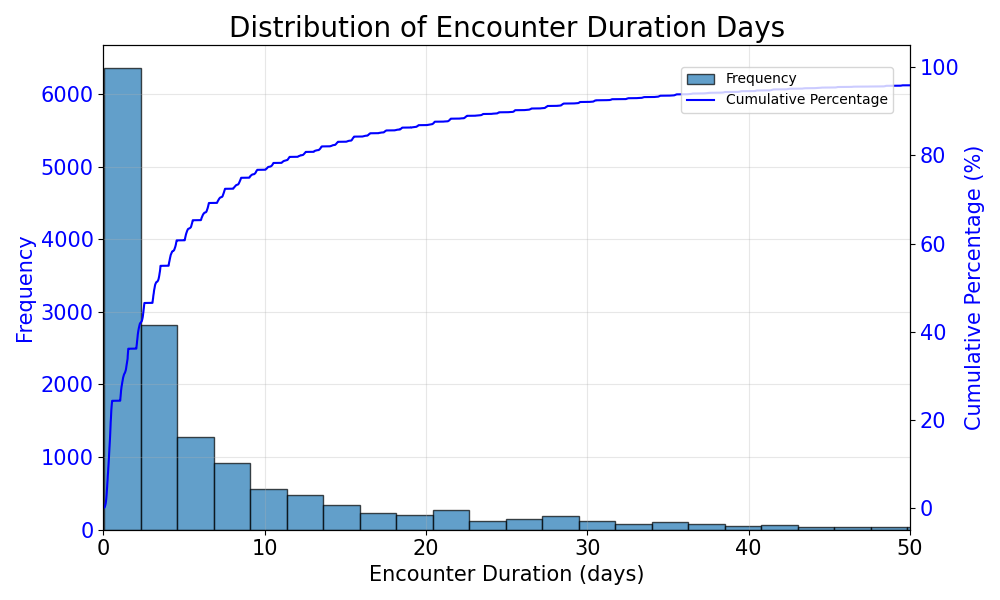
\includegraphics[width=\textwidth,height=0.72\textheight,keepaspectratio]{../figures/los/encounter_duration_days_distribution.png}
\captionof{figure}{Shows the empirical distribution of encounter duration in days, with a cumulative percentage curve to motivate the downstream long-stay and patient-load prediction task. Source: \texttt{cleaned\_models.ipynb}, cell 2.}
\end{frame}

\begin{frame}{Long-stay model ROC with additional features}
\centering
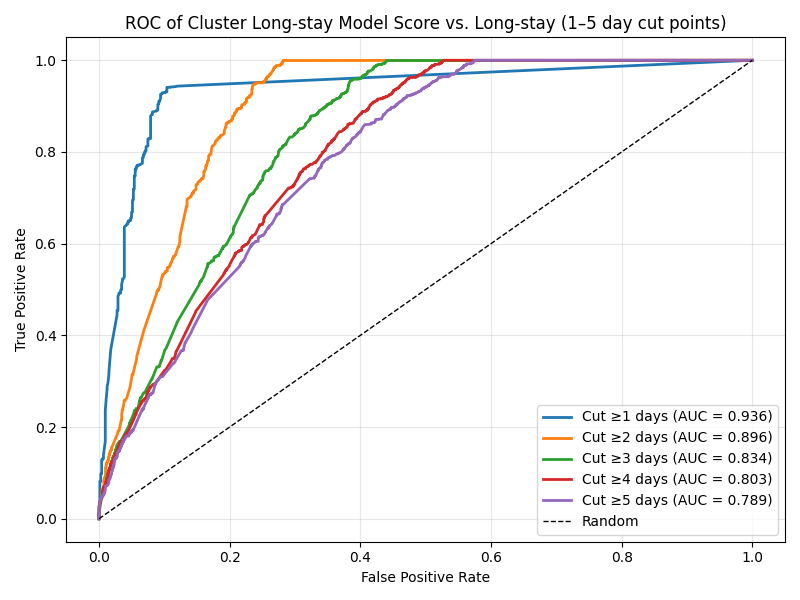
\includegraphics[width=\textwidth,height=0.72\textheight,keepaspectratio]{../figures/los/with_additional_features_roc.png}
\captionof{figure}{Summarizes discrimination for the long-stay classifiers. Source logic: \texttt{cleaned\_models.ipynb}, cells 3--7.}
\end{frame}

\begin{frame}{Long-stay model cut points with additional features}
\centering
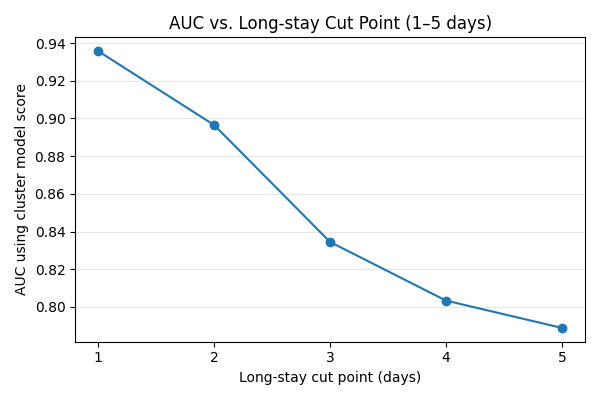
\includegraphics[width=\textwidth,height=0.72\textheight,keepaspectratio]{../figures/los/with_additional_features_cut_points.png}
\captionof{figure}{Shows operating cut points for translating long-stay probabilities into day-level workload estimates. Source logic: \texttt{cleaned\_models.ipynb}, cells 5--8.}
\end{frame}

\begin{frame}{Daily expected versus actual patient load}
\centering
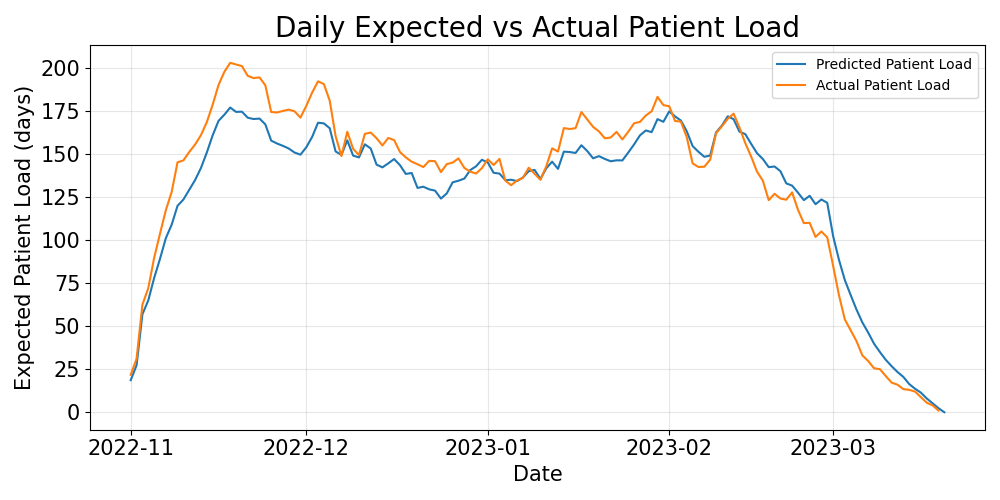
\includegraphics[width=\textwidth,height=0.72\textheight,keepaspectratio]{../figures/los/daily_expected_vs_actual_patientload.png}
\captionof{figure}{Compares expected daily patient load from summed long-stay probabilities against actual workloads reconstructed from observed encounter durations. Source: \texttt{cleaned\_models.ipynb}, cells 8, 11--12.}
\end{frame}

\begin{frame}{Actual patient load by medical service}
\centering
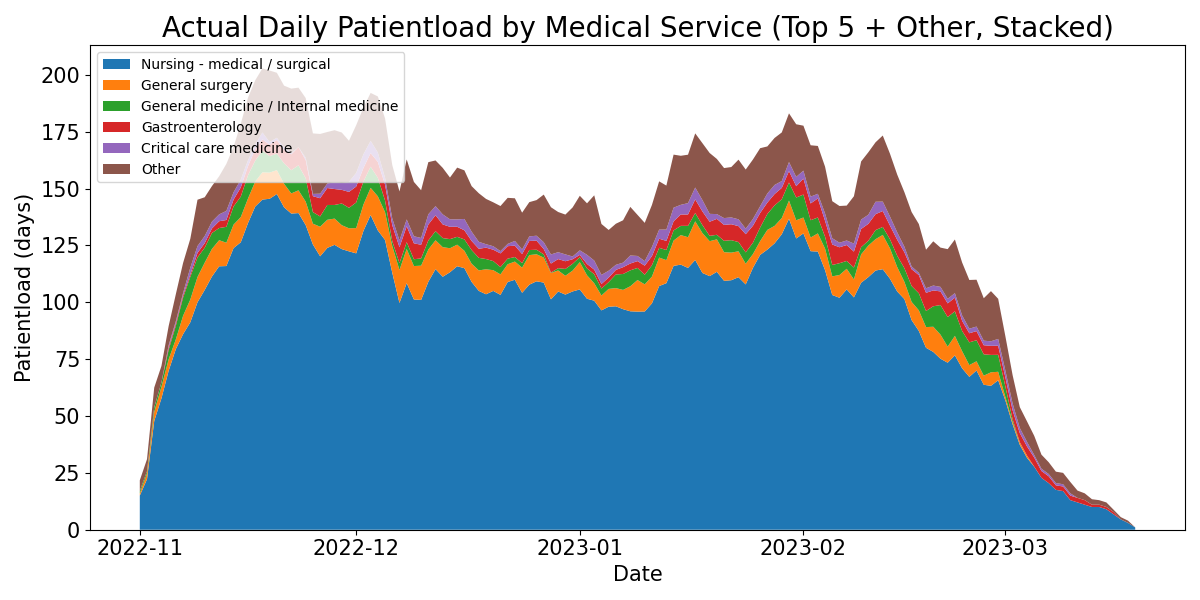
\includegraphics[width=\textwidth,height=0.72\textheight,keepaspectratio]{../figures/los/actual_daily_patientload_by_medical_service.png}
\captionof{figure}{Breaks actual daily workload into the top five medical services plus an ``Other'' category, using observed encounter duration contributions. Source: \texttt{cleaned\_models.ipynb}, cell 9.}
\end{frame}

\begin{frame}{Predicted patient load by medical service}
\centering
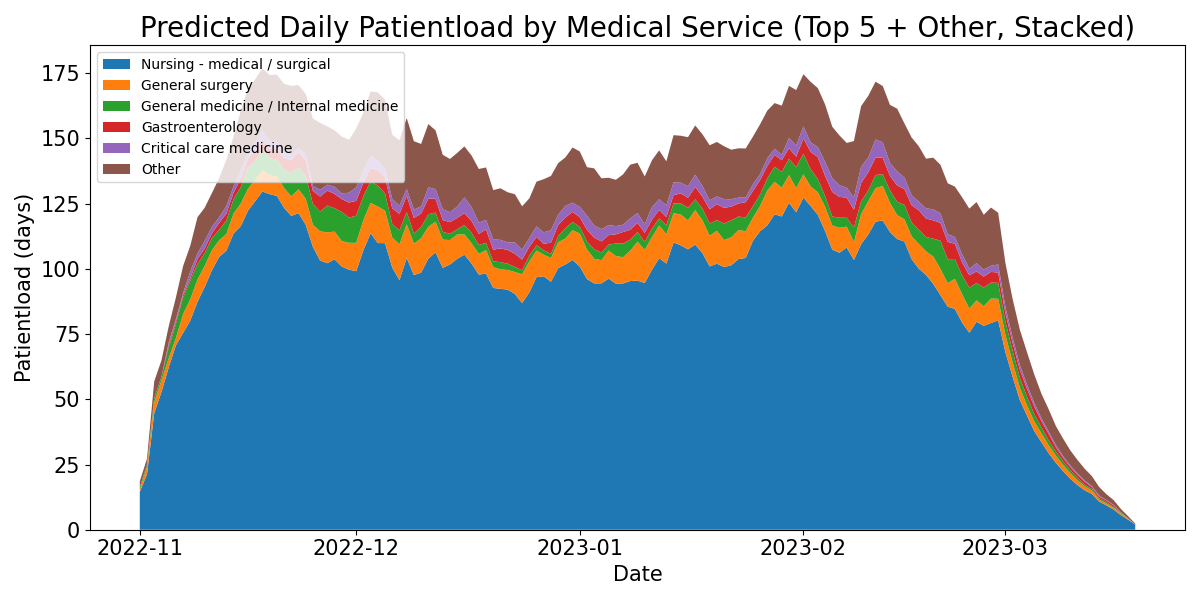
\includegraphics[width=\textwidth,height=0.72\textheight,keepaspectratio]{../figures/los/predict_daily_patientload_by_medical_service.png}
\captionof{figure}{Shows predicted daily workload by medical service by summing each encounter's probability of extending into future days. Source: \texttt{cleaned\_models.ipynb}, cell 9.}
\end{frame}

\begin{frame}{Predicted versus actual patient load by service}
\centering
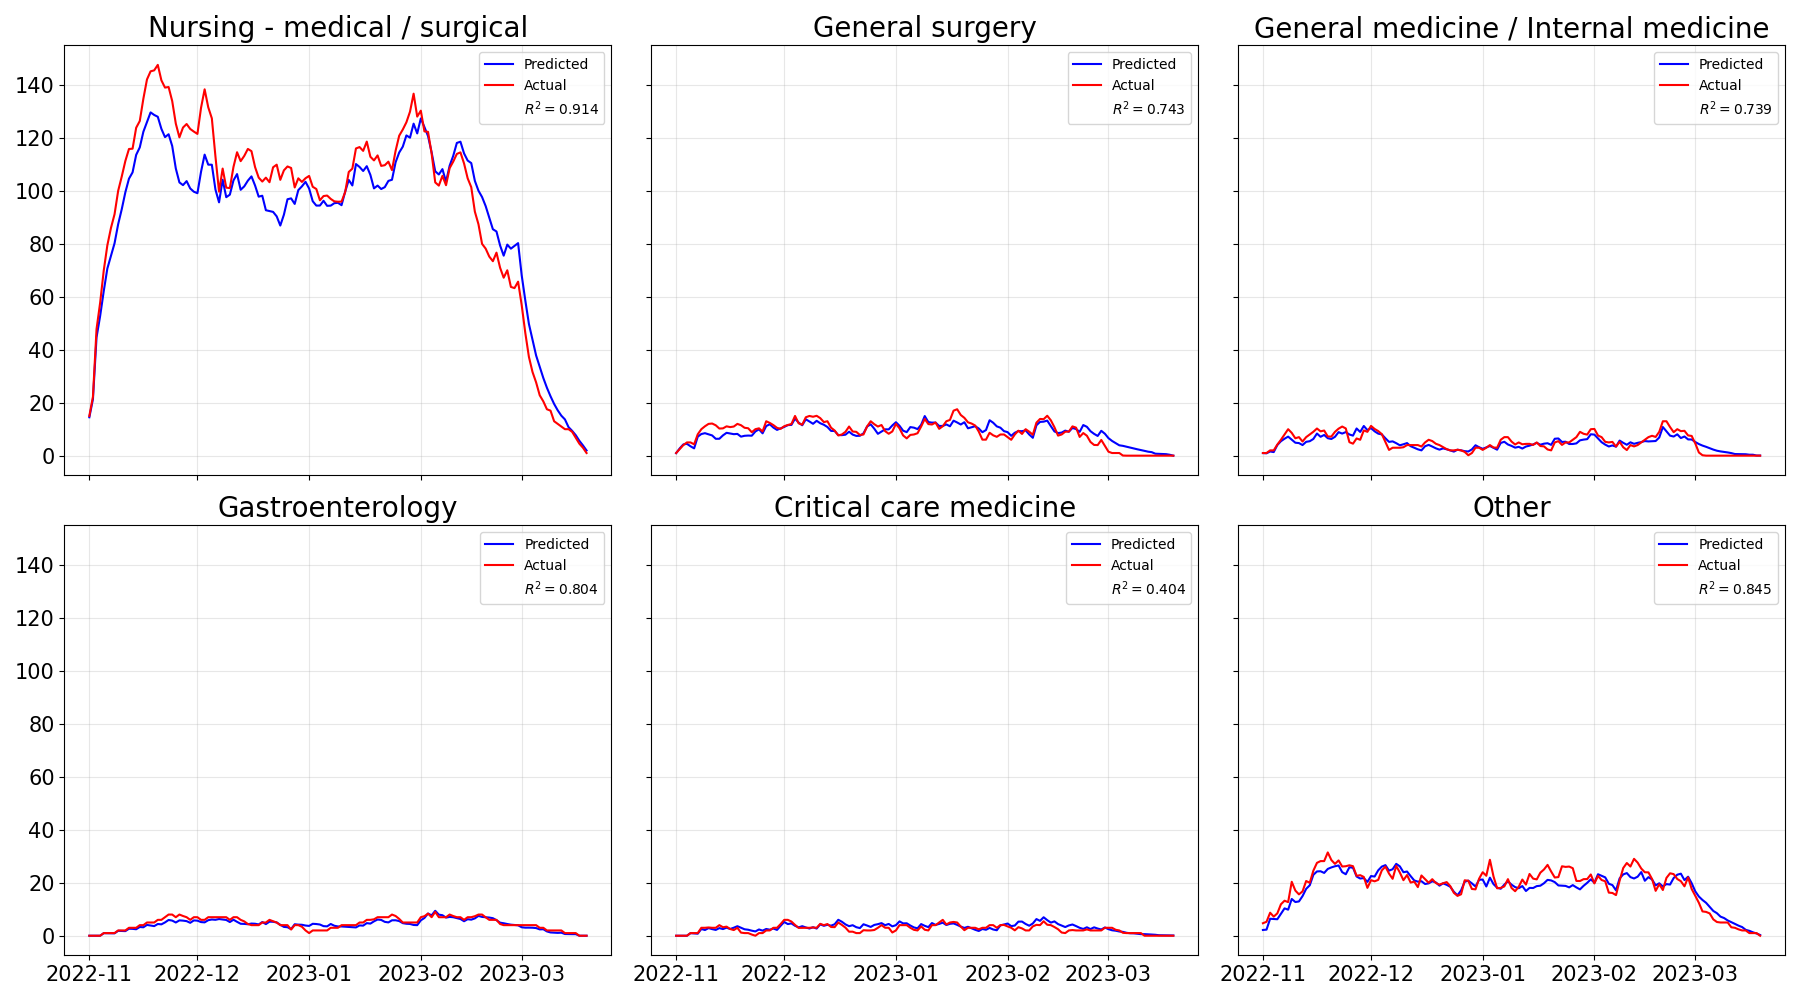
\includegraphics[width=\textwidth,height=0.72\textheight,keepaspectratio]{../figures/los/predicted_vs_actual_patientloads_by_medical_service.png}
\captionof{figure}{Compares predicted and actual service-level patient load over time, with $R^2$ reported per service panel. Source: \texttt{cleaned\_models.ipynb}, cell 10.}
\end{frame}

\section{Procedure prediction and workload}

\begin{frame}{ROC curves for top 10 procedures}
\centering
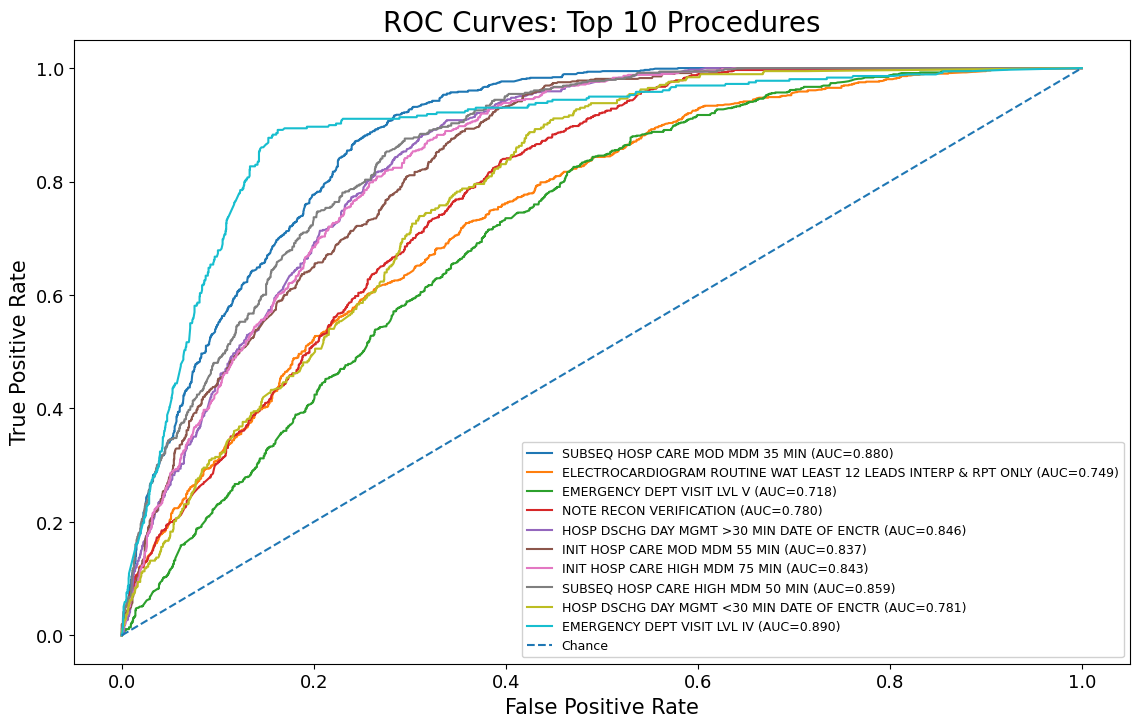
\includegraphics[width=\textwidth,height=0.72\textheight,keepaspectratio]{../figures/procedures/roc_curves_top10_procedures.png}
\captionof{figure}{Evaluates one classifier per common procedure using ROC curves and AUC values for the top ten procedure labels. Source: \texttt{procedures.ipynb}, cells 6--8.}
\end{frame}

\begin{frame}{Predicted versus actual positives for top procedures}
\centering
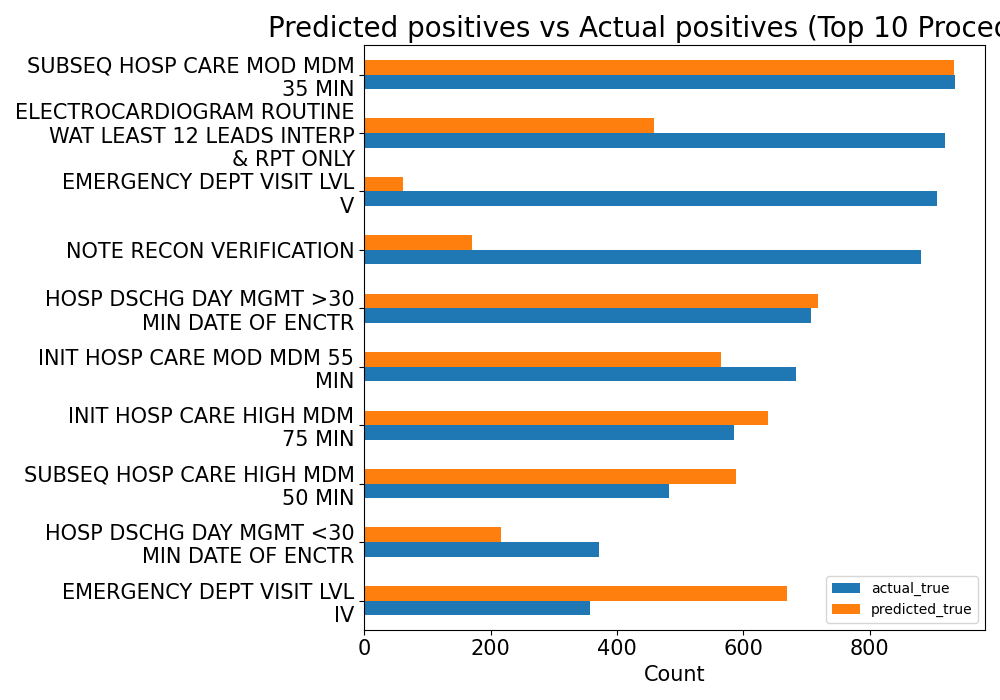
\includegraphics[width=\textwidth,height=0.72\textheight,keepaspectratio]{../figures/procedures/predicted_vs_actual_positives_top10_procedures.png}
\captionof{figure}{Compares the number of actual positive procedure labels to thresholded model predictions for the top ten procedures. Source: \texttt{procedures.ipynb}, cell 10.}
\end{frame}

\begin{frame}{Day-level procedure model ROC}
\centering
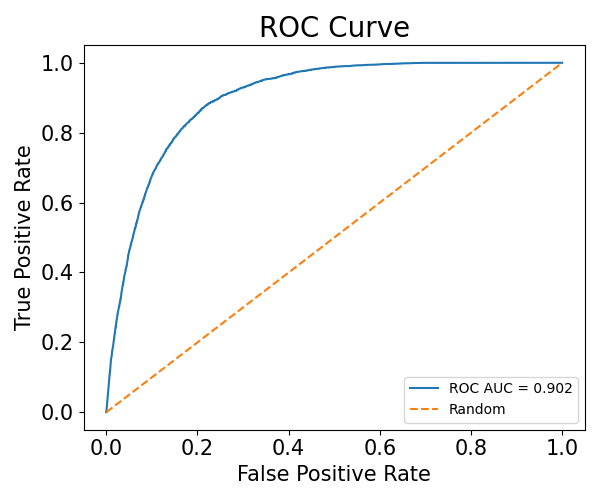
\includegraphics[width=\textwidth,height=0.72\textheight,keepaspectratio]{../figures/procedures/day_level_procedure_model_roc_curve.png}
\captionof{figure}{Evaluates the day-level procedure-occurrence model, which predicts whether selected procedures occur on a given day of an encounter. Source: \texttt{procedures.ipynb}, cells 12--13.}
\end{frame}

\begin{frame}{Day-level procedure model precision-recall}
\centering
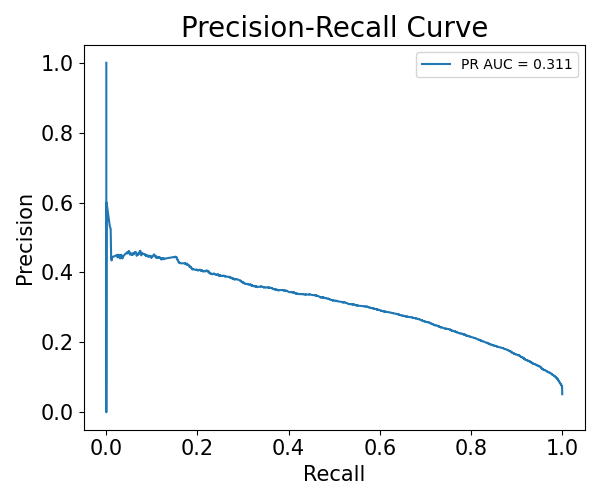
\includegraphics[width=\textwidth,height=0.72\textheight,keepaspectratio]{../figures/procedures/day_level_procedure_model_pr_curve.png}
\captionof{figure}{Evaluates precision and recall across thresholds for the day-level procedure-occurrence model. Because positive procedure days are rare, PR AUC should be interpreted relative to the positive-rate baseline. Source: \texttt{procedures.ipynb}, cells 12--13.}
\end{frame}

\begin{frame}{Procedure occurrences by encounter day}
\centering
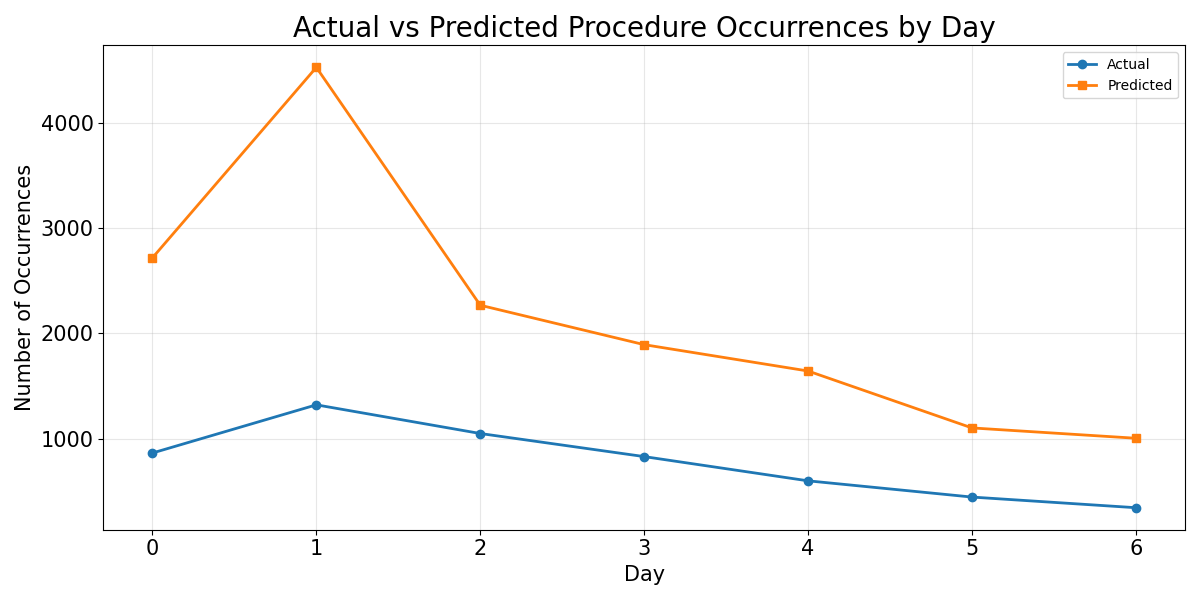
\includegraphics[width=\textwidth,height=0.72\textheight,keepaspectratio]{../figures/procedures/daily_expected_vs_actual_procedure_occurrences.png}
\captionof{figure}{Aggregates actual and predicted procedure occurrences by encounter day to show whether the model captures within-stay procedure timing. Source: \texttt{procedures.ipynb}, cell 14.}
\end{frame}

\begin{frame}{Procedure occurrence counts by calendar day}
\centering
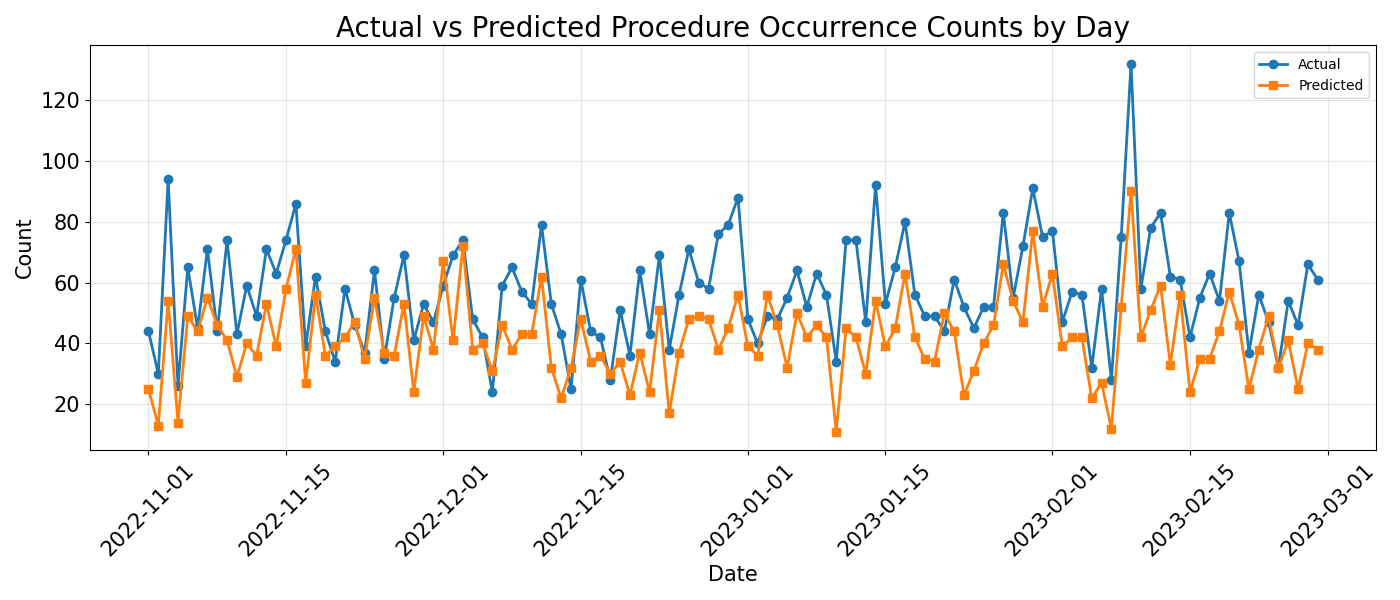
\includegraphics[width=\textwidth,height=0.72\textheight,keepaspectratio]{../figures/procedures/daily_expected_vs_actual_procedure_occurrence_counts.png}
\captionof{figure}{Compares daily actual versus predicted counts of top-ten procedure occurrences using encounter start dates. Source: \texttt{procedures.ipynb}, cell 16.}
\end{frame}

\begin{frame}{Procedure occurrences by encounter start date}
\centering
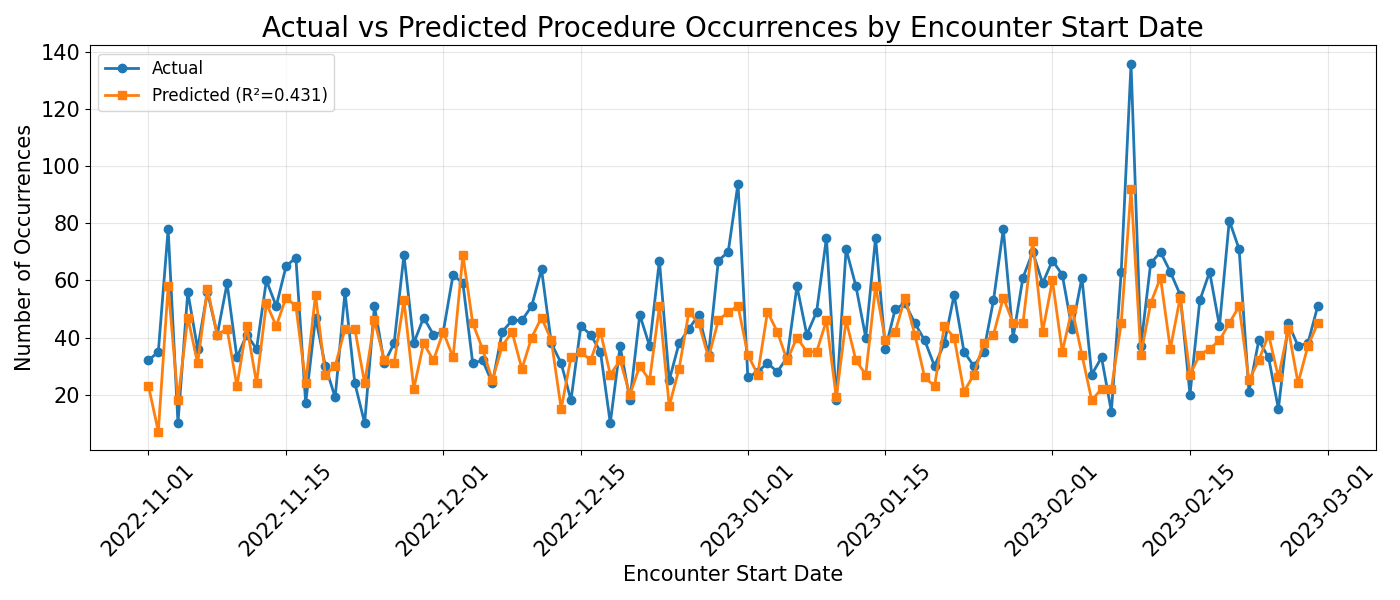
\includegraphics[width=\textwidth,height=0.72\textheight,keepaspectratio]{../figures/procedures/daily_expected_vs_actual_procedure_occurrences_by_encounter_start_date.png}
\captionof{figure}{Shows actual and predicted procedure occurrences over encounter start dates, including an $R^2$ summary for temporal fit. Source: \texttt{procedures.ipynb}, cell 17.}
\end{frame}

\begin{frame}{Estimated procedure time by day}
\centering
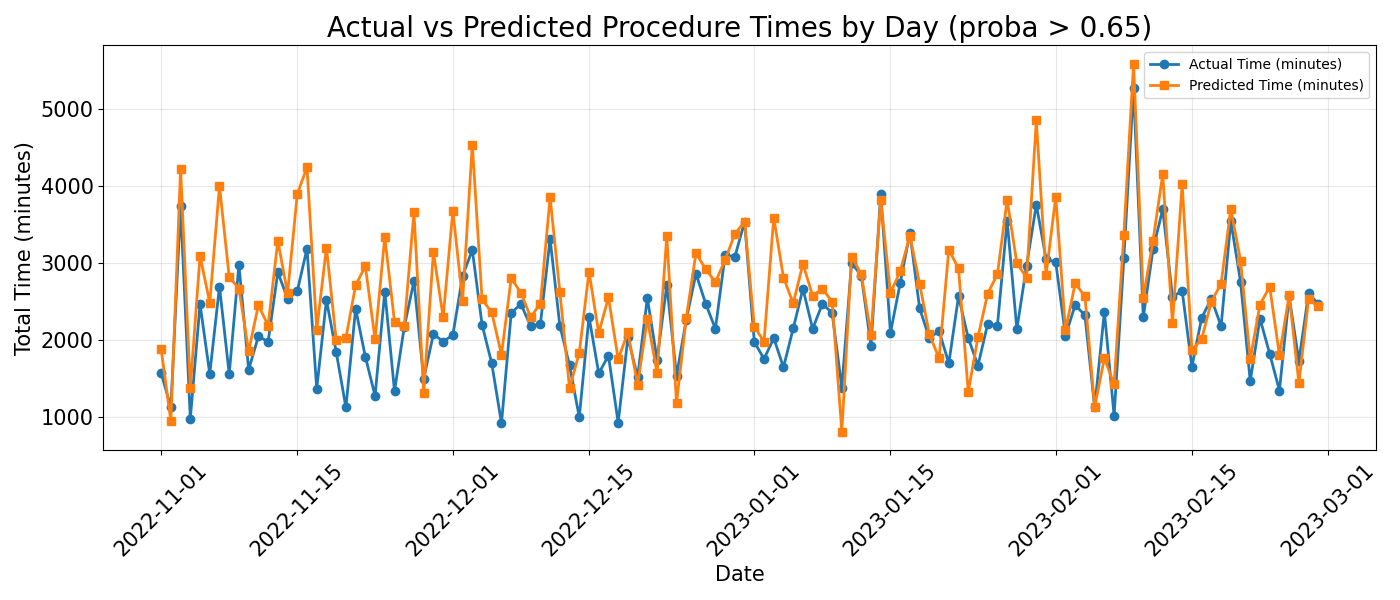
\includegraphics[width=\textwidth,height=0.72\textheight,keepaspectratio]{../figures/procedures/daily_expected_vs_actual_procedure_times.png}
\captionof{figure}{Converts predicted and actual procedure labels into estimated minutes using a hand-coded procedure-time dictionary, then aggregates by day. Source: \texttt{procedures.ipynb}, cells 24--26.}
\end{frame}

\end{document}